\chapter{The Minimal Supersymmetric Standard Model}\label{ch:supersymmetry}

Historically, examining nature at increasing energy scales (and correspondingly decreasing length scales ) has consistently yielded new physics. For example, higher-energy experiments were able to probe the structure of the weak interactions, precisely at the energy scale that the 4-Fermi theory started to fail. Similarly, the challenges listed at the end of \autoref{ch:sm} most likely point to new physics at higher energy scales, between the currently explored weak scale to the reduced Planck scale:
\begin{equation*}
M_P = 1/\sqrt{8\pi G} \approx 2.4\times 10^{18} \text{ GeV}
\end{equation*}
However, the SM Higgs potential is extremely sensitive to new physics at high energies. The mass of the SM Higgs boson receives large quantum corrections from any new physics at high energies that couples to the Higgs sector. For example, if the Higgs couples to a heavy fermion \emph{f} through a term of the form $-\lambda_fH\bar{f}f$, the one-loop correction to the higgs mass (\autoref{fig:one_loop_fermion}) takes the form
\begin{equation}
\Delta m_H^2 = -\frac{|\lambda_f|^2}{8\pi^2}\Lambda_\text{UV}^2 + ...
\label{eq:one_loop_fermion}
\end{equation}
\begin{marginfigure}
\feynmandiagram [layered layout, horizontal=b to c] { 
  a [particle=\(h\)] -- [scalar] b -- [fermion, half left, edge label=\(f\)] c -- [fermion, half left] b, c -- [scalar] d,
};
\caption{Feynman diagram for the one-loop fermionic correction to the SM Higgs mass}
\label{fig:one_loop_fermion}
\end{marginfigure}
where $\Lambda_{UV}$ is some cutoff momentum where the effects of the new physics are expected to manifest themselves. Similarly, the one-loop correction from a heavy scalar \emph{S} through the term $-\lambda_S|H|^2|S|^2$ (\autoref{fig:one_loop_scalar}) takes the form
\begin{equation}
  \Delta m_H^2 = \frac{\lambda_S}{16\pi^2}\left[\Lambda_\text{UV}^2 + ...\right]
\label{eq:one_loop_scalar}
\end{equation}
\begin{marginfigure}
\begin{tikzpicture}
\begin{feynman}
  \vertex (a){\(h\)};
	\vertex [right=of a] (b);
	\vertex [right=of b] (c);
    \vertex [above=of b] (d);
\diagram*{
	{
      [edges = scalar]
      (a) -- (b) -- (c),
      (b) -- [half left, edge label=\(S\)] (d) -- [half left] (b),
    },
};
\end{feynman}
\end{tikzpicture}
\caption{Feynman diagram for the one-loop scalar correction to the SM Higgs mass}
\label{fig:one_loop_scalar}
\end{marginfigure}
\strictpagecheck
In both these cases, the size of the correction scales quadratically with the momentum cutoff $\Lambda_{UV}$. Higher-order loop corrections can be shown to be similarly large as well. Thus the `natural' mass of the Higgs would seem to be on the the order of $\Lambda_{UV}$, which could even be as high as the Planck scale. In contrast, the actual mass that we measure is only about 126 GeV. Thus there is a \emph{hierarchy} between the observed and the `natural' mass of the SM Higgs, one of many orders of magnitude. \footnote{Note that even though only the mass of the SM Higgs is directly sensitive to $\Lambda_{UV}$, this sensitivity is propagated to all the other SM particles through their couplings to the SM Higgs.}
Thus it would seem that any UV completion of the SM would have to come with a host of parameters to tune the counterterms enough to cancel out the quadratic divergences and result in the physical mass we observe experimentally. If the new physics is at the Planck scale, the divergences must cancel to less than one part in $10^{-16}$ to give us a SM Higgs at the weak scale.
It is obviously undesirable to have to manually tune a large number of parameters to be able to come up with UV completions of the Standard Model - it would be analogous to the geocentric Ptolemaians adding an ever-increasing number of epicycles to explain what would ultimately be more simply and accurately described by Copernicus's heliocentric theory. 
Looking at the forms of the one-loop corrections in \eqref{eq:one_loop_fermion} and \eqref{eq:one_loop_scalar}, we can see that the contribution from the fermion \emph{f} will be exactly canceled out by the contributions from two complex scalars \footnote{Thus also matching the number of fermionic and scalar degrees of freedom.} with $\lambda_S = |\lambda_f|^2$, the corrections from the scalar and the fermion will cancel out exactly. This suggests that the simplest way to ensure that all quadratic divergences from new physics at high energy scales cancel out is to require some kind of symmetry between fermions and scalars, ensuring that there is a scalar partner for each fermion, or vice versa.

This symmetry is known as \emph{supersymmetry}. It is a rich mathematical structure with far-reaching consequences, a lot of which are beyond the scope of this work. For a pedagogical review of supersymmetry, we refer the reader to \citep{Martin1997}. This section provides a necessarily condensed version of the treatment there. 
The term `supersymmetry' refers to the invariance of the Lagrangian under supersymmetry transformations of the form\footnote{Of course, this is not the precise form of the transformation - as can be seen by performing some rudimentary dimensional analysis. We write done more precise transformations later.}
\begin{align*}
  Q|\text{Boson}\rangle = |\text{Fermion}\rangle &&\text{and}&& Q|\text{Fermion}\rangle = |\text{Boson}\rangle.
\end{align*}

The minimal phenomenologically viable supersymmetric extension to the Standard Model is known as the \emph{Minimal Supersymmetric Standard Model}, or the MSSM. Although the hierarchy problem has been the main driving force behind the development of supersymmetry, there are other benefits that the MSSM provides as well.
One of them is that the MSSM has the right particle content to unify the strong and electroweak couplings at a high energy scale, as seen in \autoref{fig:gauge_coupling_unification}.

\begin{marginfigure}[-4cm]
    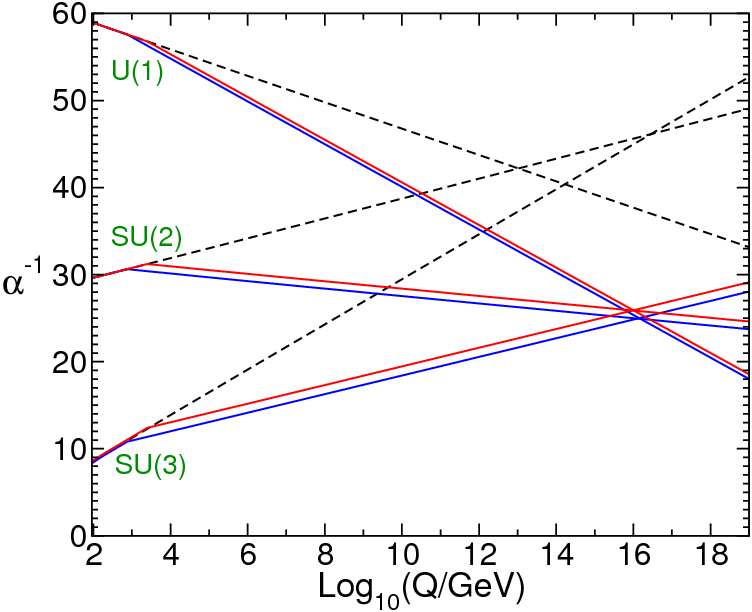
\includegraphics[width=\textwidth]{images/gauge_coupling_unification}
  \caption{2-loop RG evolution of inverse gauge couplings in the SM (dashed lines) and the MSSM (solid lines). The sparticle masses are varied between 0.5-1.5 TeV, and $\alpha_3(m_Z)$ is varied between 0.117 and 0.121. Source: \citep{Martin1997}.}
  \label{fig:gauge_coupling_unification}
\end{marginfigure}

The third major motivation (and the one most relevant to this dissertation) is the fact that the MSSM results in a viable dark matter candidate. The MSSM admits a new kind of discrete symmetry known as \emph{R-parity}. It is an analogue of baryon and lepton number conservation. The Lagrangian of the MSSM is defined to be invariant under the action of the operator $P_R$ on the fields. The eigenvalues of this operator are $(-1)^{3(B-L)+2s}$, where \emph{B, L}, and \emph{s} represent the baryon number, lepton number, and spin of the particle, respectively. The consequence of this is that the lightest supersymmetric particle (LSP) must be absolutely stable, that is, it cannot decay further into other particles, thus making it a good candidate for particle dark matter.

However, before describing the salient features of the MSSM, we will outline the construction of a general supersymmetric Lagrangian with all the necessary ingredients we need: kinetic terms, mass terms, scalar self-interactions, gauge symmetry, and Yukawa interactions, and then specialize to the MSSM.

\section{Chiral and gauge supermultiplets}
Having seen what Lagrangians with supergauge symmetry look like in the superfield and superspace formulation, we can recover regular scalar, vector and spinor fields that are functions of the bosonic coordinates by Taylor expanding the superfields in the Lagrangian. Consider the expansion of a chiral superfield given by
\[\Phi(y,\theta) = \phi(y) + \sqrt{2}\theta\psi(y)+\theta\theta F(y).\]
Choosing values of $\phi,\psi,$ and \emph{F} fixes $\Phi$. Thus, they can be grouped naturally into an object called a \emph{supermultiplet}. In this case, we say that the fields $\phi,\psi,$ and \emph{F} reside in a \emph{chiral} supermultiplet, and that $\phi$ and $\psi$ are superpartners of each other. Recall that an infinitesimal supersymmetry transformation mixes fermionic and bosonic degrees of freedom. Generically, the scalar partner of a fermion is referred to as a \emph{sfermion}. Similarly, recall the expansion of a vector superfield in the Wess-Zumino gauge:
\[V_\text{Wess-Zumino gauge} = \bar{\theta}\bar{\sigma}^\mu\theta A_\mu+\bar{\theta}\bar{\theta}\theta\lambda+\theta\theta\bar{\theta}\lambda^\dagger+\frac{1}{2}\theta\theta\bar{\theta}\bar{\theta}D\]
The fields $A_\mu,\lambda,$ and \emph{D} form another natural grouping, called a \emph{vector} supermultiplet. The fields $A_\mu$ and $\lambda$ are superpartners of each other, and fields such as $\lambda$ are generically known as \emph{gauginos}\footnote{After the co-inventor of the Wess-Zumino model, Bruno Zumino.}.
Let us now take a superpotential of the form:
\begin{equation}
W = \frac{1}{2}M^{ij}\Phi_i\Phi_j + \frac{1}{6}y^{ijk}\Phi_i\Phi_j\Phi_k
\label{eq:superpotential}
\end{equation}
where $M$ is a mass matrix, and $y$ represents the Yukawa couplings and scalar self-interactions.
If we expand the superfields in terms of the component fields, and integrate out the auxiliary fields \emph{F} and \emph{D}, we end up with
\begin{align*}
  \mathcal{L} &= \overbrace{-D^\mu\phi^{\dagger i}D_\mu\phi_i + i\psi^{\dagger i}\bar{\sigma}^\mu D_\mu\psi_i}^\text{kinetic terms}
  -\overbrace{\frac{1}{2}\left\{M^{ij}\psi_i\psi_j+\text{h.c.}\right\}}^{\text{fermion mass terms}}
   +\overbrace{M_{ik}^*M^{kj}\phi^{*i}\phi_j}^\text{scalar mass terms}\\
  &-\overbrace{\frac{1}{2}\left\{y^{ijk}\phi_i\psi_j\psi_k+\text{h.c.}\right\}}^{\text{Yukawa terms}}
  +\overbrace{\frac{1}{2}\left\{M^{in}y_{jkn}^*\phi_i\phi^{*j}\phi^{*k}+\text{h.c.}\right\}}^\text{scalar cubic interactions}\\
  &+\overbrace{\frac{1}{2}g_a^2(\phi^{\dagger i}(T^a)_i^j\phi_j)^2+\frac{1}{4}\left\{y^{ijn}y_{kln}^*\phi_i\phi_j\phi^{*k}\phi^{*l}\right\}}^\text{scalar quartic interactions}\\
  &-\overbrace{\frac{1}{4}F_{\mu}^aF^{\mu\nu a}}^\text{gauge boson self-interactions}
  +\overbrace{i\lambda^{\dagger a}\bar{\sigma}^\mu D_\mu\lambda^a}^\text{gaugino-gauge boson interactions}
\end{align*}
The MSSM has analogues of all of the above terms.

\section{Softly broken supersymmetry}
The component fields of a superfield have the same mass, as can be seen from the mass terms above. This means that, if supersymmetry holds, the superpartners of the SM particles should have been discovered by now. Evidently, if this symmetry exists, it is not evident in the ground state that we inhabit - that is, it must be spontaneously broken. The exact mechanism by which it is broken is still unknown - there are a number of competing models which introduce new physics at high energy scales. To remain model-agnostic, we can simply perform a parameterized explicit breaking by inserting the relevant terms into the Lagrangian by hand. The form of these terms is constrained by the requirement that the quadratic divergences in the radiative corrections to scalar masses must still vanish. With this constraint, we can write a set of generic soft SUSY-breaking terms:

\section{The Minimal Supersymmetry Standard Model}

Specifying a collection of chiral supermultiplets, the gauge symmetry structure, a superpotential of the form in \eqref{eq:superpotential}, and a set of soft SUSY-breaking terms should be enough to reproduce a supersymmetric Lagrangian like the one above. With that in mind, let us put together the ingredients of the MSSM. The first is a gauge symmetry structure, which we will take to be the same as the Standard Model:
\begin{equation*}
  SU(3)_c\times SU(2)_L\times U(1)_Y
\end{equation*}
The next is a set of chiral supermultiplets, and the gauge supermultiplets that correspond to our gauge symmetry structure. These supermultiplets define the particle content of the theory. We show them in \autoref{tab:chiral_supermultiplets} and \autoref{tab:gauge_supermultiplets}, grouped by which group representation they transform under. For brevity, we have not shown all three fermion generations.
\begin{table}
  \caption{Chiral supermultiplets of the MSSM.}
  \label{tab:chiral_supermultiplets}
  \begin{tabular}{cccccc}
    \toprule
                   & \multicolumn{2}{c}{Components}                  & \multicolumn{3}{c}{Group representation} \\ \cmidrule(r){2-3}\cmidrule(l){4-6}
    Superfield     & Spin-0                                          & Spin-$\slantfrac{1}{2}$                                                        & $SU(3)_c$          & $SU(2)_L$    & $U(1)_Y$\\\midrule
                   & Squarks                                         & Quarks                                                                         &                    &              & \\ \cmidrule(r){2-3}\\
    Q              & $\vdoublet{\widetilde{u}_L}{\widetilde{d}_L}$   & $\vdoublet{u_L}{d_L}$                                                          & $\mathbf{3}$       & $\mathbf{2}$ & $\frac{1}{2}$\\\\
    $\overline{u}$ & $\tilde{u}_R^*$                                 & $u_R^\dagger$                                                                  & $\bar{\mathbf{3}}$ & $\mathbf{1}$ & -$\frac{2}{3}$\\\\
    $\overline{d}$ & $\tilde{d}_R^*$                                 & $d_R^\dagger$                                                                  & $\bar{\mathbf{3}}$ & $\mathbf{1}$ & $\frac{1}{3}$\\\\\cmidrule{2-3}
                   & Sleptons                                        & Leptons                                                                        &                    &              & \\ \cmidrule{2-3}\\
    \emph{L}       & $\vdoublet{\widetilde{\nu}_L}{\widetilde{e}_L}$ & $\vdoublet{\nu_L}{e_L}$                                                        & $\mathbf{1}$       & $\mathbf{2}$ & -$\frac{1}{2}$\\\\
    $\overline{e}$ & $\tilde{e}_R^*$                                 & $e_R^\dagger$                                                                  & $\bar{\mathbf{1}}$ & $\mathbf{1}$ & $1$\\\\\cmidrule{2-3}
                   & Higgses                                         & Higgsinos                                                                      &                    &              & \\ \cmidrule{2-3}\\
    $H_u$          & $\vdoublet{H_u^+}{H_u^0}$                       & $\vdoublet{\widetilde{H}_u^+}{\widetilde{H}_u^0}$                              & $\mathbf{1}$       & $\mathbf{2}$ & $\frac{1}{2}$\\\\
    $H_d$          & $\vdoublet{H_d^0}{H_d^-}$                       & $\vdoublet{\widetilde{H}_d^0}{\widetilde{H}_d^-}$                              & $\mathbf{1}$       & $\mathbf{2}$ & -$\frac{1}{2}$\\\\
    \bottomrule
  \end{tabular}
\end{table}

\begin{table}
  \caption{Gauge supermultiplets of the MSSM.}
  \label{tab:gauge_supermultiplets}
  \begin{tabular}{ccccc}
    \toprule
\multicolumn{2}{c}{Components} & \multicolumn{3}{c}{Group representation} \\ \cmidrule(r){1-2}\cmidrule(l){3-5}
Spin-$\slantfrac{1}{2}$        & Spin-1                                                                         & $SU(3)_c$          & $SU(2)_L$    & $U(1)_Y$\\\midrule
Gluinos: $\widetilde{g}$       & Gluons: \emph{g}                                                               & $\mathbf{8}$       & $\mathbf{1}$ & 0 \\\\
Winos: $\widetilde{W}^0$       & W bosons: $W^\pm$                                                              & $\bar{\mathbf{1}}$ & $\mathbf{3}$ & 0\\\\
Binos: $\widetilde{B}^0$       & B bosons: $B^0$                                                                & $\bar{\mathbf{1}}$ & $\mathbf{3}$ & 0\\
    \bottomrule
  \end{tabular}
\end{table}
Next, let us specify the superpotential. In terms of the chiral superfields in \autoref{tab:chiral_supermultiplets}, we can write the MSSM superpotential as:
\[W_\text{MSSM} = \bar{u}\mathbf{y_u}QH_u-\bar{d}\mathbf{y_d}Q H_d-\bar{e}\mathbf{y_e}L H_d+\mu H_u H_d \]
where we have abbreviated terms such as $\mu(H_u)_\alpha (H_d)_\beta\epsilon^{\alpha\beta}$ to $\mu H_u H_d$, and the matrices $\mathbf{y}$ are $3\times3$ matrices of Yukawa couplings, with indices representing the fermion generations. 
Note also that we now see the necessity of having two Higgs doublets - one that couples to the up-type fermions, and the other to the down-type fermions. A term like $\overline{u}\mathbf{y_u}QH_d^*$ would lead to a non-conserved hypercharge.
Finally, we have a set of terms that soft SUSY-breaking terms\footnote{\Adarsh{Note to self: explain the tilde notation.}}.
\begin{align*}
  \begin{split}
    \mathcal{L}_\text{soft}^\text{MSSM} = &-\frac{1}{2}\left(M_1\widetilde{B}\widetilde{B}+
    M_2\widetilde{W}\widetilde{W} + M_3\widetilde{g}\widetilde{g} + \text{h.c.}\right)\\
    &-\left(\widetilde{\overline{u}}\mathbf{a_u}\widetilde{Q}H_u-\widetilde{\overline{d}}\mathbf{a_d}-\widetilde{\overline{e}}\mathbf{a_e}\widetilde{L}H_d+\text{h.c.}\right)\\
    &-\widetilde{Q}^\dagger\mathbf{m_Q^2}\widetilde{Q}
     -\widetilde{L}^\dagger\mathbf{m_L^2}\widetilde{L}
     -\widetilde{\overline{u}}^\dagger\mathbf{m_{\overline{u}}^2}\widetilde{\overline{u}}^\dagger
     -\widetilde{\overline{d}}^\dagger\mathbf{m_{\overline{d}}^2}\widetilde{\overline{d}}^\dagger
     -\widetilde{\overline{e}}^\dagger\mathbf{m_{\overline{e}}^2}\widetilde{\overline{e}}^\dagger\\
     &-m^2_{H_u}H^*_uH_u-m^2_{H_d}H_d^*H_d-(bH_uH_d+\text{h.c.}) 
  \end{split}
\end{align*}
\subsection{Phenomenological approximations}
Often, the MSSM has a number of simplifying assumptions motivated both by convenience and compatibility with observed experimental data. For example, it is convenient to take the Yukawa matrices $\mathbf{y_u,y_d,y_e}$ in a simplified limit, where only the heaviest generations have non-zero Yukawa couplings. 
\begin{align*}
  \mathbf{y_u} \approx \begin{pmatrix}
    0 & 0 & 0\\
    0 & 0 & 0\\
    0 & 0 & y_t
  \end{pmatrix},&&
  \mathbf{y_d} \approx \begin{pmatrix}
    0 & 0 & 0\\
    0 & 0 & 0\\
    0 & 0 & y_b
  \end{pmatrix},&&
  \mathbf{y_e} \approx \begin{pmatrix}
    0 & 0 & 0\\
    0 & 0 & 0\\
    0 & 0 & y_\tau
  \end{pmatrix}
\end{align*}
Furthermore, to suppress excessive CP-violation and FCNCs in the MSSM, the following approximations are often made. First, we assume that there is minimal mixing among the sfermions:
\begin{align*}
  \mathbf{m_Q^2} = m_Q^2\mathbf{1},&&
  \mathbf{m_{\bar{u}}^2} = m_{\bar{u}}^2\mathbf{1},&&
  \mathbf{m_{\bar{d}}^2} = m_{\bar{d}}^2\mathbf{1},&&
  \mathbf{m_{\bar{e}}^2} = m_{\bar{e}}^2\mathbf{1},&&
  \mathbf{m_{\bar{L}}^2} = m_{\bar{L}}^2\mathbf{1}\\
\end{align*}
We also suppress the cubic scalar couplings of the first two families of sfermions by imposing the conditions: 
\begin{align*}
  \mathbf{a_u} = A_{u0}\mathbf{y_u},&&
  \mathbf{a_d} = A_{d0}\mathbf{y_d},&&
  \mathbf{a_e} = A_{e0}\mathbf{y_e}.\\
\end{align*}
Finally, requiring that the soft SUSY breaking parameters are real enables us to suppress excessive amounts of CP violation:
\begin{align*}
  \text{Im}(M_1)=
  \text{Im}(M_2)=
  \text{Im}(M_3)=
  \text{Im}(A_{u0})=
  \text{Im}(A_{d0})=
  \text{Im}(A_{e0})=0.
\end{align*}
With the above ingredients, one can work out myriad phenomenological consequences. In \autoref{ch:DM_100_TeV}, we examine the neutralino sector of the MSSM in slightly more detail.
